%%%%%%%%%%%%%%%%%%
% 			 
%			Master Thesis - UWB
%				Introduction code
%
%			Author : Wilson Daubry
%
%%%%%%%%%%%%%%%%%%

\chapter{Introduction}
\pagenumbering{arabic} 
\setcounter{page}{1}
\label{introduction}

Nowadays, indoor localization is a growing feature of many smart buildings, either to allow the navigation of autonomous robots, navigate in an unknown building using an indoor version of the \gls{gps}, etc. The widespread \gls{gps} is not suited for indoor localization \cite{bejuri2013ubiquitous} \cite{kulmer2017using}. In this scope, an indoor locating system using the \gls{uwb} technology and based on trilateration has been fastened in \cite{hannotier2019indoor}.
\vspace{2mm}

This locating system finds the position of a mobile device, called tag using three beacons, named anchors, set at known position. The schematic of this system is shown in Fig. \ref{fig:schem_loc}. The tag, mainly consists in an \gls{uwb} antenna and a smartphone with a custom android application developed to display the position and orientation of the tag on a given map.

\begin{figure}[H]
\centering
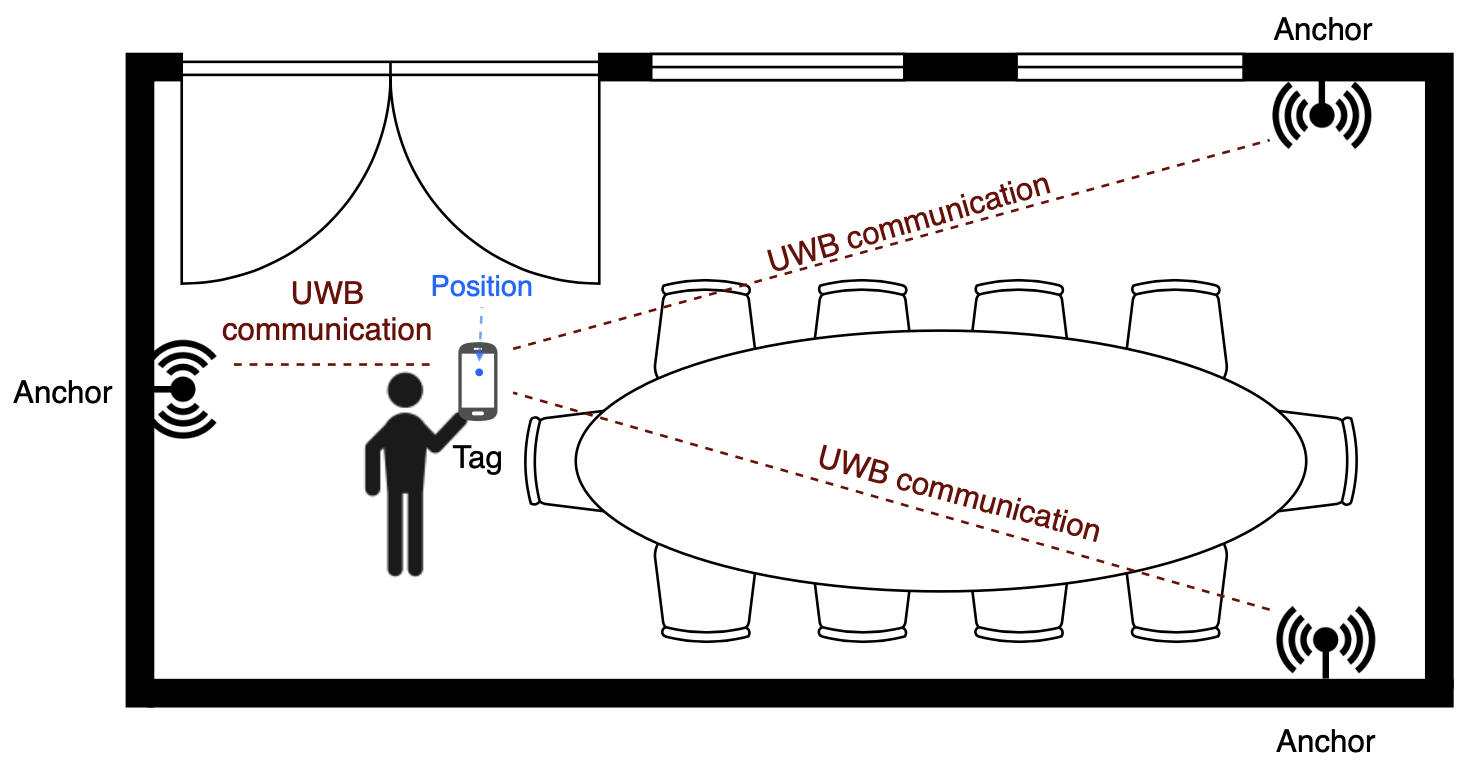
\includegraphics[width=.8\linewidth]{Images/schem_loc.png}
\caption{Schematic of an indoor locating system, a tag interacting with three anchor to know its position in the room. Taken from \cite{hannotier2019indoor}.\label{fig:schem_loc}}
\end{figure}

This locating system is based on the assumption that a \gls{los} between the tag and the anchor is always clear, no object or body obstructing it. Since this can not be guaranteed for every location, at every moment, for indoor location, two main possibilities occur. The first is to increase the number of available anchors, statistically increasing the probability to always have two \gls{los}. This approach has been studied in \cite{guyard2019navigation}. The second approach, is to develop a locating system that may function with less than three antennas available. This thesis focuses on this second approach, studying and qualifying a locating system using only one anchor.
\vspace{2mm}

In the second chapter, a state of the art is displayed, summarizing the previous work made about \gls{uwb}, \gls{rtls}, indoor locating systems, describing the functioning of the locating system implemented in \cite{hannotier2019indoor} and detailing the theory behind some 'one anchor'  locating systems. In the third chapter, two different algorithms developed to perform the indoor localization using only one anchor are shown.
\vspace{2mm}

Chapter four focuses on the simulation developed to test and study the algorithms developed in chapter \ref{algos}. The functioning of the simulation is first used and the simulation results of the two algorithms are then shown. The fifth chapter focuses on the implementation and modification of the experimental set-up in order to test and extract experimental data to test the algorithms in a real environment.
\vspace{2mm}

The last chapter comes back to the work carried out and the results obtained during this thesis, outlining the research topics that should be investigated in further work, concluding this thesis.
\vspace{2mm}

\subsubsection{Message to the reader}

Before reading this thesis, the reader must be warned that the last section will seem rather unfinished. Because of the COVID-19 virus situation and the resulting lock-down, the experiment part, which was supposed to be the main focus of this thesis, was compromised. From that moment, the scope of the thesis was reorientated towards simulations that should be as realistic as possible in order to lead the same sort of analysis as would have been done using experimental data.